The problem presented here was originally proposed by Batsui Mitsunao, a fifteen-year-old boy, and written on a tablet hung in 1812 at the Nishihirokami Hachiman shrine in Izumi city, Toyama prefecture, Japan (Fukagawa Hidetoshi and Tony Rothman, \textit{Sacred Mathematics: Japanese Temple Geometry}, Princeton University Press, 2008). 

Several circles of radius $r$ are packed to form a pyramid, using $n$ circles along each side, as shown in the figure below in the special case $n=4$. A larger circle circumscribes the pyramid. Express the radius of the larger circle in terms of $r$ and $n$. Express the ratio of the areas of the $n$ smaller circles to the area of the larger circle in terms of $n$. Calculate the limit of the ratio as $n\rightarrow\infty$. 

\begin{figure}[H]
\centering
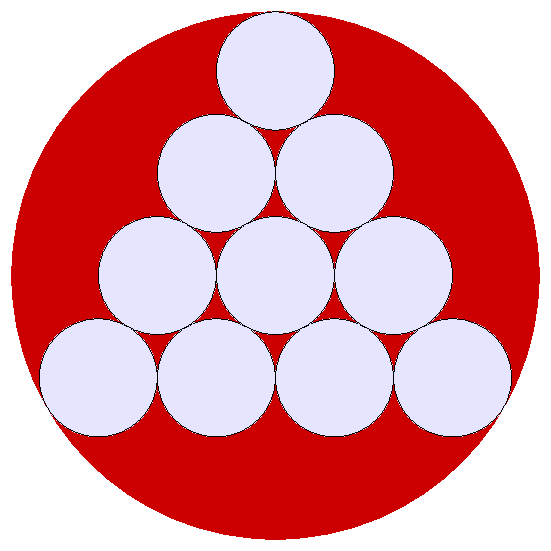
\includegraphics[height=6cm,page=1]{circles-in-pyramid}
\end{figure}
